\documentclass[aspectratio=169]{beamer}

\usepackage{tikzducks}

\setbeamertemplate{navigation symbols}{}
\setbeamertemplate{background canvas}{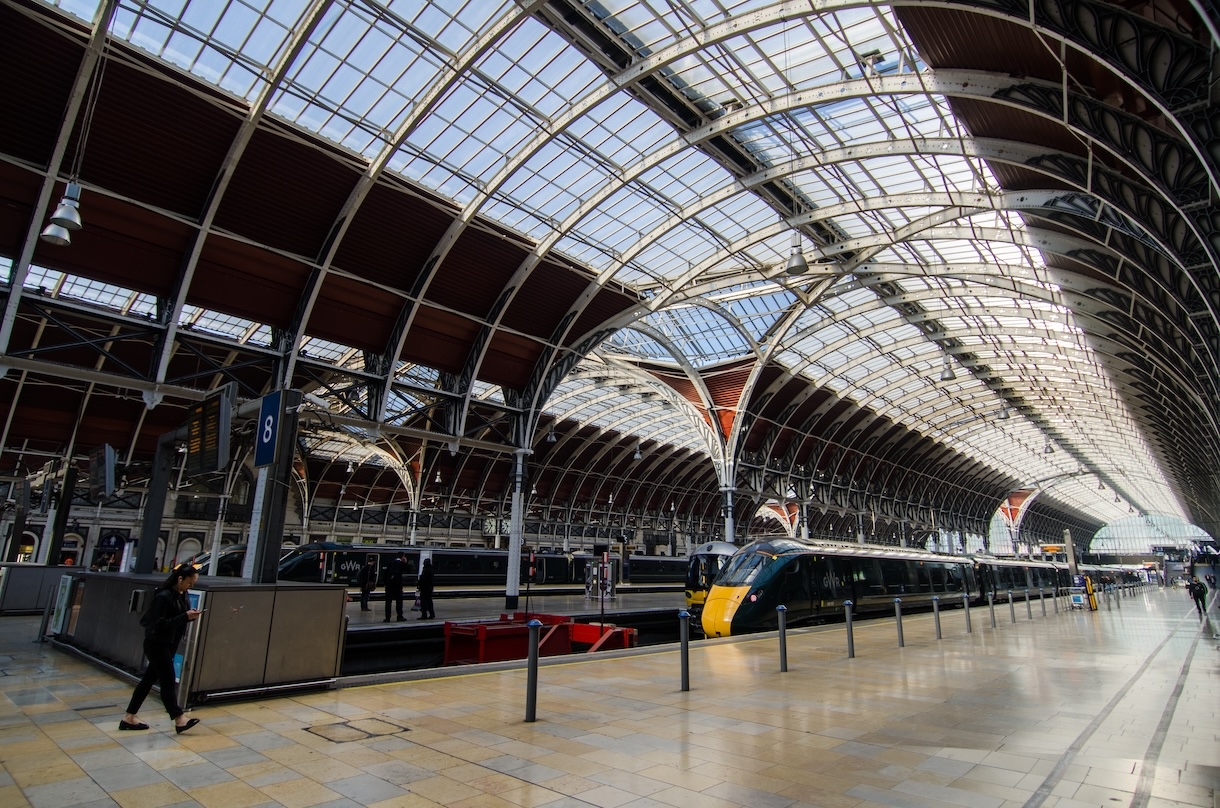
\includegraphics[width=\paperwidth]{Paddington_Station_GWR}}
\graphicspath{{include/}}

% trick taken from https://topanswers.xyz/tex?q=1989
\tikzset{
    use page relative coordinates/.style={
        shift={(current page.south west)},
        x={(current page.south east)},
        y={(current page.north west)}
    },
}

\usepackage{xfp}
\ExplSyntaxOn
\let\intmodnn\int_mod:nn
\ExplSyntaxOff

\begin{document}

\begin{frame}
  \begin{tikzpicture}[remember picture, overlay,use page relative coordinates]
  
    \ifnum \intmodnn{\thepage}{10} > 5
      \node at (0.75,0.28) {
\includegraphics[height=5cm]{paddi}};
    \else
      \node at (0.75,0.28) {
\includegraphics[height=5cm]{paddi2}};
    \fi

    % credit for background image
    \node[white,text width=.9\paperwidth,font=\tiny,align=center] at ([yshift=0.35cm]current page.south) {Image by @Jeff Hitchcock \href{https://creativecommons.org/licenses/by/2.0/deed.en}{CC BY 2.0} 
    (\url{https://en.wikipedia.org/wiki/File:Paddington_Station_GWR.jpg})
    };

  \end{tikzpicture}
  \pause[300]
\end{frame}

\end{document}